\chapter{Improving flexibility of macros}
\label{improving-flexibility-macros}

\todo[inline]{Explain the old macro system with an example. Q: Isn't that the section below already?}



\section{Explanation of the macro system}

% What are the limitations without macros?
% Most importantly: syncats. gf-ud assumes that every word is in a leaf, represented by a lexical gf-function. however, syncategorimatic words \todo{define?} (or functions?) come from the functions that are used to combine trees (what are those called?) and would be missing otherwise. E.g. "is" is syncategorimatic in gf for english, because there is no lexical function for copula, because not all languages use a word for copula. So we make up a lexical gf-function for "is", which is then combined with a made-up version of MkCl which is converted into the thing we need.
% This is terrible writing!

In order to overcome some limitations \todo{(which?)} of the conversion there is a system of macros. A macro is an imaginary GF function that will get converted into an expression of real GF functions after the conversion step of gf2ud is done.

% Syncats?

When one GF function corresponds to multiple different dependency labels, a macro can be used to disambiguate which one is meant without losing the information

Example from \cite{kolachina-ranta-2017}



% We noted in Section 2 that ud2gf has to deal with
% ambiguity, incompleteness, noise, and ungrammaticality. The basic algorithm of Section 3 takes
% none of these aspects into account. But it does
% contain what is needed for ambiguity: the list ts
% of previous trees at each node can also be used
% more generally for storing alternative trees. The
% “main” tree t is then compared and ranked together with these candidates. Ranking based on
% tree probabilities in previous GF treebanks, as in
% (Angelov, 2011), is readily available. But an even
% more important criterion is the node coverage of
% the tree. This means penalizing heavily those trees
% that don’t cover all nodes in the subtrees.
% This leads us to the problem of incompleteness:
% what happens if the application of all possible candidate functions and trees still does not lead to a
% tree covering all nodes? An important part of this
% problem is due to syncategorematic words. For
% instance, the copula in GF is usually introduced as
% a part of the linearization, and does not have a category or function of its own.6 To take the simplest
% possible example, consider the adjectival predication function and its linearization:
% fun UseAP : AP -> VP
% lin UseAP ap = \\agr => be agr ++ ap
% where the agreement feature of the verb phrase is
% passed to an auxiliary function be, which produces
% the correct form of the copula when the subject
% is added. The sentence the cat is black has the
% following tree obtained from UD:





\begin{verbatim}
#auxfun MkVPS_Perf have vp : Have -> VP -> VPS = MkVPS (TTAnt AAnter 
  TPres) PPos vp ; aux[Tense=Pres] head
\end{verbatim}

\section{Intro to macros}

% Motivate need for auxfuns and auxcats

GF trees are on a higher abstraction level than UD trees. In UD, every token is associated with a dependency label. In contrast, any production rule in a GF grammar may introduce new tokens. This difference complicates the mapping between the two formalisms.

When introducing the problem and its partial solution, \cite{kolachina-ranta-2017} name as examples copulas, negations, tense auxiliaries and infinitive marks. We reproduce their example of the English copula (the verb “to be”) and its treatment in \verb|ud2gf|.

Figures \ref{fig:gf_cute} and \ref{fig:ud_cute} show the difference between GF’s and UD’s treatment of copulas. In the UD tree, the copula has a category and a dependency label \verb|cop|. In the GF tree, there is no special category: the string “is” is introduced by the function \verb|UseComp : AP -> VP| rule, which makes an AP into a predicate.

% \begin{figure}
%     \centering
%     \includegraphics{}
%     \caption{Caption}
%     \label{fig:enter-label}
% \end{figure}

result from \verb+p -cat=Cl "this cat is small"  | vp -view=open -showfun+:

% Produced using: https://maryszmary.github.io/ud-annotatrix//standalone/annotator.html
% And pressing the printer icon to select latex

\begin{figure}
    \centering
    % \includegraphics{}
    \begin{dependency}
       \begin{deptext}[column sep=0.4cm]
             this \& cat \& is \& small \\
           {\tt DET}\&{\tt NOUN}\&{\tt AUX}\&{\tt ADJ}\\
       \end{deptext}
       \depedge{2}{1}{det}
       \depedge{4}{2}{nsubj}
       \depedge{4}{3}{cop}
    \end{dependency} \\
    \caption{The phrase ``This cat is small'' analysed as a UD tree}
    \label{fig:enter-label}
\end{figure}

As a solution, \verb|ud2gf| introduced the notion of \emph{auxiliary categories} and \emph{auxiliary functions} in the labels file. This consists of the following parts:
\begin{itemize}
    \item Auxiliary category for copula: \verb|Cop_ VERB lemma=be|
    \item Auxiliary function that recognises the auxiliary category: \\
           \verb|UseAP_ : Cop_ -> AP -> VP ; cop head|
    \item Rule to replace the auxiliary function with an actual GF function: \\
          \verb|UseAP_ cop ap = UseAP ap|
\end{itemize}

However, coordination was still a problem in \verb|ud2gf|. The auxiliary categories and functions were not expressive enough to transform a structure like ``the small, cute and fluffy cat'' from UD to GF.





\section{Intro to flexibility problem}

As an example of a phrase that can be difficult to convert using the old gf2ud, let us consider the adjectival phrase ``cute, fluffy and furry''
would be described in UD format as in Figures \ref{fig:ud_cute_text} and \ref{fig:ud_cute}.


\begin{figure}
    \begin{verbatim}
    1  cute  cute  ADJ  JJ  Degree=Pos  0  root  _  FUN=cute_A
    2  ,  ,  PUNCT  ,  _  3  punct  _  _
    3  fluffy  fluffy  ADJ  JJ  Degree=Pos  1  conj  _  FUN=fluffy_A
    4  and  and  CCONJ  CC  _  5  cc  _  FUN=and_Conj
    5  furry  furry  ADJ  JJ  Degree=Pos  1  conj  _  FUN=furry_A
    \end{verbatim}
    % \begin{tabular}{|c|c|c|c|c|c|c|c|c|c|}
    % \hline
    % 1 & cute & cute & ADJ & JJ & Degree\=Pos & 0 & root & \_ & FUN\=cute\_A \
    % \hline
    % 2 & , & , & PUNCT & , & \_ & 3 & punct & \_ & \_ \
    % \hline
    % 3 & fluffy & fluffy & ADJ & JJ & Degree\=Pos & 1 & conj & _ & FUN\=fluffy\_A \
    % \hline
    % 4 & and & and & CCONJ & CC & \_ & 5 & cc & \_ & FUN\=and\_Conj \
    % \hline
    % 5 & furry & furry & ADJ & JJ & Degree\=Pos & 1 & conj & \_ & FUN\=furry\_A \
    % \hline
    % \end{tabular}
    \caption{The phrase ``cute, fluffy and furry'' as a textual UD tree}
    \label{fig:ud_cute_text}
\end{figure}

\begin{figure}
    \centering
    % \begin{dependency}
  \begin{deptext}[column sep=0.4cm]
      cute \& , \& fluffy \& and \& furry \\
    {\tt ADJ}\&{\tt PUNCT}\&{\tt ADJ}\&{\tt CCONJ}\&{\tt ADJ} \\
  \end{deptext}
  \depedge{2}{1}{punct}
  \depedge{0}{2}{conj}
  \depedge{4}{3}{cc}
  \depedge{0}{4}{conj}
\end{dependency} \\
    % \includesvg{ud-annotatrix-corpus.svg}
    % 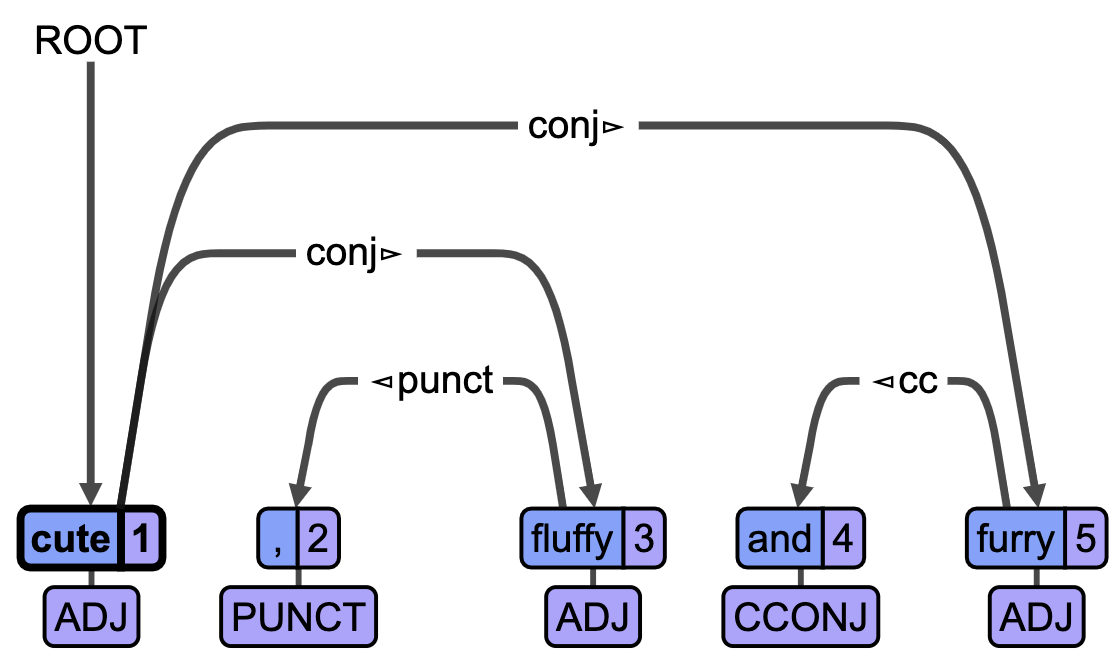
\includegraphics[width=0.7\textwidth]{figure/ud_cute.png}
    \begin{dependency}
        \begin{deptext}[column sep=0.4cm]
              cute \& , \& fluffy \& and \& furry \\
            {\tt ADJ}\&{\tt PUNCT}\&{\tt ADJ}\&{\tt CCONJ}\&{\tt ADJ}\\
        \end{deptext}
        \depedge{3}{2}{punct}
        \depedge{1}{3}{conj}
        \depedge{5}{4}{cc}
        \depedge{1}{5}{conj}
    \end{dependency} \\
    \caption{The phrase ``cute, fluffy and furry'' as a UD tree in graphical format}
    \label{fig:ud_cute}
\end{figure}
% \include{}

\begin{figure}
    \centering
    % \begin{dependency}
  \begin{deptext}[column sep=0.4cm]
      cute \& , \& fluffy \& and \& furry \\
    {\tt ADJ}\&{\tt PUNCT}\&{\tt ADJ}\&{\tt CCONJ}\&{\tt ADJ} \\
  \end{deptext}
  \depedge{2}{1}{punct}
  \depedge{0}{2}{conj}
  \depedge{4}{3}{cc}
  \depedge{0}{4}{conj}
\end{dependency} \\
    % \includesvg{ud-annotatrix-corpus.svg}
    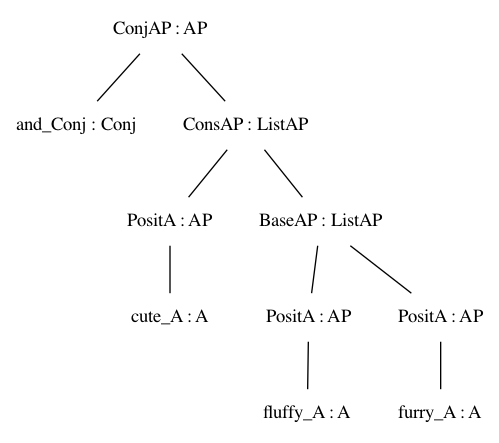
\includegraphics[width=0.7\textwidth]{figure/cute_gf.png}
    \caption{The phrase ``cute, fluffy and furry'' as a GF tree in graphical format. }
    \label{fig:gf_cute}
\end{figure}

The GF version of the same tree, shown in Figure \ref{fig:gf_cute}, would look like this:

\begin{verbatim}
ConjAP and_Conj (ConsAP (PositA cute_A)
                        (BaseAP (PositA fluffy_A) (PositA furry_A)))
\end{verbatim}
Here we can see that in UD, the word ``cute'' is in the root, while the conjunction ``and'' is at the bottom of the tree, while in GF the conjunction is a direct child of the root. This transformation can not be preformed by the simple single-layer transformations that are available in the current macro-system for labels files.



\section{Thing}

Most of the time the structure in UD trees are similar enough to allow a fairly direct translation.
There are however some difficult cases where the structure is significantly different in a way that was impossible to overcome using the old macro system.

One such example is when you have a series of conjunctions, for example the phrase:

  small, fluffy, furry and cute

In 

\section{Ideas for further improvements}

A more structured implementation of this could be to add (anonymous) records to the syntax of macros similar to the concrete syntax of GF. 